%%%%%%%%%%%%%%%%%%%%%%%
\chapter{システムテストにおけるブラックボックステストの課題}
本研究は,ソフトウェアテストの中で,システムテストレベルでのブラックボックステストを研究対象にする.ブラックボックステストのテストケースを開発するプロセスの中では,テスト分析を対象にする.本章では,これら研究対象の定義を説明し,そこで起きている課題を述べる.

\newpage
\section{テストケースの開発方法とテストのレベル}
\subsection{アプリケーションソフトウェアの構成}
本研究では,図\ref{fig:fig-1}に示す状態$St$と保持データ$Ds$を持つアプリケーションソフトウェア$AS$に対するソフトウェアテストを研究対象にする.アプリケーションソフトウェア$AS$は,入力$In$に対して,何らかの出力$Out$を返す.
ソフトウェアの機能は,何らかの入力$In$を出力$Out$に変換する処理により実現されていると考えられる.
この処理を本研究ではタスク$Ta$と呼ぶ.
タスク$Ta$は,該当のテストレベルからみた入力を出力に変換している1処理である.
そのため,タスク$Ta$のサイズは,テストレベルによって決まる.
ユニットテストのレベルであれば関数となり,システムテストのレベルであれば,システムを利用するユーザが操作する機能で行われる処理となる.
ソフトウェアの構成要素であるタスク$Ta$の出力$Out$について考えると,$Ta$への入力$In$だけでなく状態$St$と保持データ(データベースや内部メモリに保存されているデータ)$Ds$の影響を受けると考えられる.
例えば,Webアプリケーションにて予約を行うタスク$Ta$について考えると,予約が可能か否かを示す状態$St$と,予約オブジェクトの予約状況を示す保持データ$Ds$によって予約の成否が決まる.

%−−−-図1を入れる
\begin{figure}[H]
  \begin{center}
  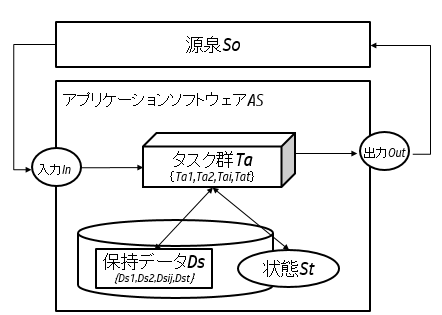
\includegraphics[width=11cm]{./image/fig-1.png}
  \caption{アプリケーションソフトウェアの構成}
  \label{fig:fig-1}
  \end{center}
\end{figure}

アプリケーションソフトウェア$AS$の構成要素は,タスク群$Ta$と状態$St$と保持データ$Ds$とし,外部の源泉$So$からの入力$In$と$So$への出力$Out$があるとする.
タスク群$Ta$は,その要素を$Ta=\{Ta_1,Ta_2,\cdots,Ta_i,\cdots,Ta_t \}$とし, 対応する入出力は$In_i$と$Out_i$とする.
\subsection{ホワイトボックステストとブラックボックステスト}
テストケースの種類は,ソフトウェアの物理的な構造を基にテスト設計をするホワイトボックステストと,ソフトウェアの仕様を基にテスト設計をするブラックボックステストに大別できる\cite{myers2011art} .

\begin{figure}[htbp]
  \begin{center}
  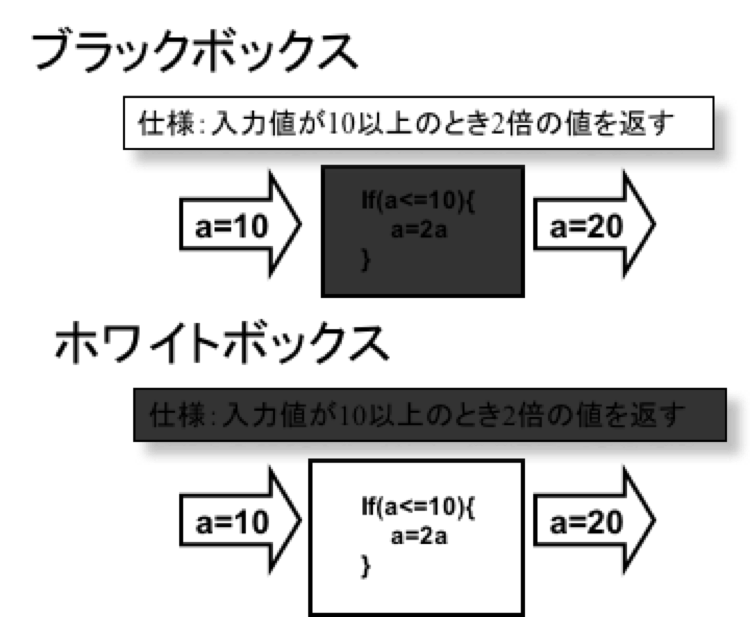
\includegraphics[width=10cm]{./image/BlackboxWhitebox.png}
  \caption{ホワイトボックステストとブラックボックステストの違い}
  \label{fig:D-2-Fig0}
  \end{center}
\end{figure}

ホワイトボックステストとブラックボックステストの違いを図~\ref{fig:D-2-Fig0}に示す.
両者の違いはテストの網羅基準とテストケースの抽出方法の違いである.
ホワイトボックステストは,テスト設計のベースがテスト対象となる$AS$の内部要素である$Ta$の構造になる.
ユニットテストのレベルで例えると,$Ta$の内部構造となるプログラムのソースコードの行を網羅,分岐を網羅するように$In$を与えて$Out$を確認するといったように,網羅すべきアイテムを明確に選択してテストケースを開発する.
網羅基準はテスト設計技法として提唱されている\cite{myers2011art}\cite{beiz90}\cite{copeland2004practitioner}.

一方,ブラックボックステストは,テスト対象そのものではなく,$Ta$に対する動作条件や振る舞いについて記述した仕様をベースにしてテストケースを開発する.
ブラックボックステストのテスト設計技法では,仕様に対する網羅基準が数多く提唱されている\cite{jorgensen2016software}\cite{binder2000testing}\cite{kaner1999testing}\cite{black2007pragmatic}.

しかし,ブラックボックステストは,テスト設計のベースがテスト対象の物理的な構造ではなく論理的なふるまいの記述であるがゆえに,テストを作るための詳細化が複数の解釈で行われることが多い.
複数の解釈で行う結果として,テストケースの重複や抜け漏れを引き起こす可能性も高くなる.

本研究では,テストケースの設計方法の種類はブラックボックステストを対象とする.

\subsection{テストレベル}

ソフトウェアテストは,開発ライフサイクルの中で複数のテストレベルに分けて行われる.
複数のテストレベルは,図~\ref{fig:D-2-Fig1}で示すVモデルと呼ばれる技術面にフォーカスしたライフサイクルモデルにて表現することができる\cite{forsberg}.
テストレベルは,ソフトウェア開発の段階的詳細化のレベルと対応している\cite{pressman2005software}.

\begin{figure}[htbp]
  \begin{center}
  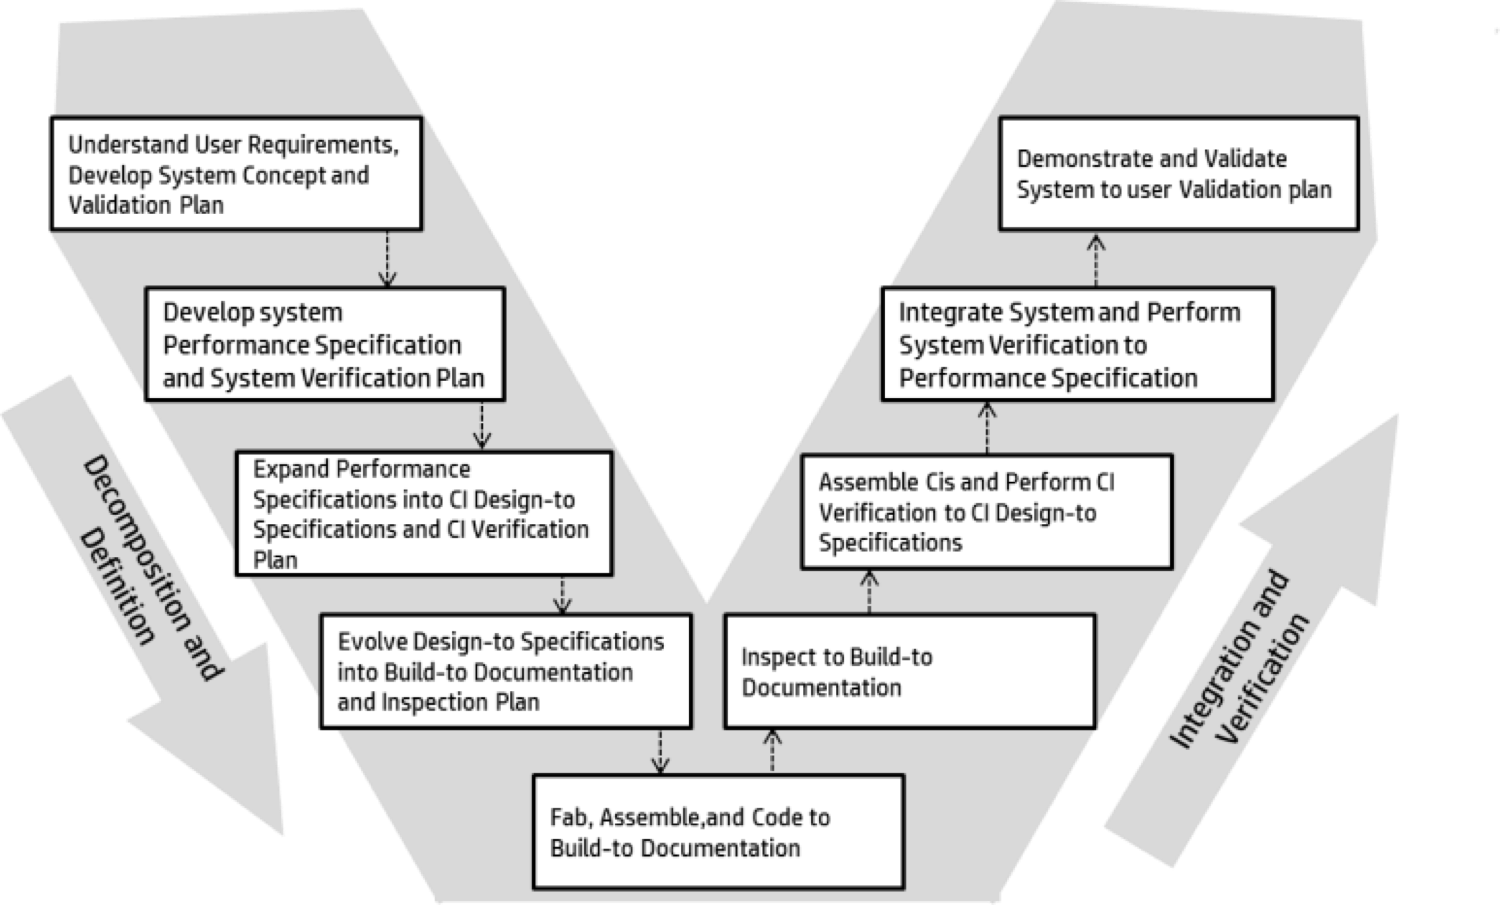
\includegraphics[width=12cm]{./image/D-2-Fig1.png}
  \caption{Vモデル}
  \label{fig:D-2-Fig1}
  \end{center}
\end{figure}

テストのプロセスは,Vモデルであらわす各レベルごとに行われる.
本研究は,複数のテストレベルの中で,図~\ref{fig:D-2-Fig1}の上から2番目の箱となる,「Develop System performance specification and System verification plan」と「Integration system and Perform system verification to performance specificetion」のレベル,つまりシステムテストのレベルで実行するブラックボックステストに焦点を当てている.
システムテストのレベルは,開発した単体のソフトウェアがすべて統合されるため,規模の増大と複雑性の増加の影響を直接的に受けるからである.

\subsection{テスト開発プロセス}
Vモデルであらわす各レベルにて行われるテストは,それぞれ開発プロセスと類似したプロセスを持っている.
テストのプロセスは, 図~\ref{fig:D-2-Fig2}のようにテスト計画がVモデルの左側の活動と並行に行われ,その後時系列にテスト分析,テスト設計,テスト実装が行われた後,Vモデルの右側の活動の中で,テスト実行と終了基準の評価が行われる.
\begin{figure}[htbp]
  \begin{center}
  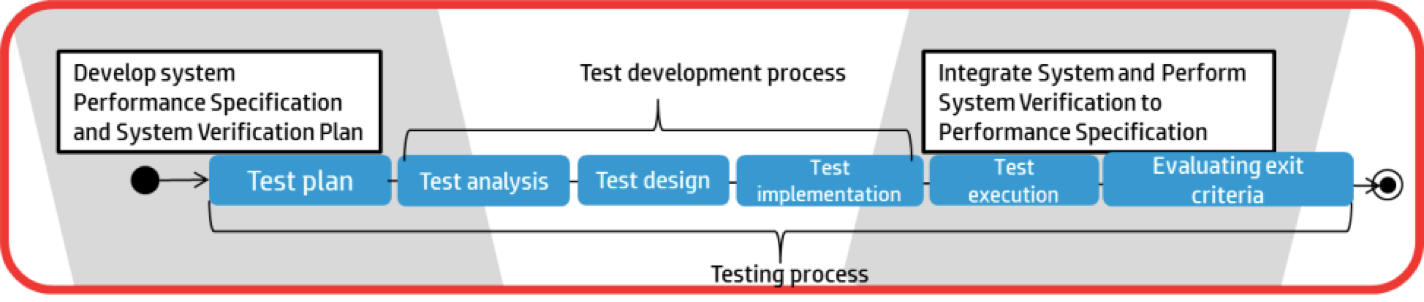
\includegraphics[width=14cm]{./image/D-2-Fig2.png}
  \caption{テスト開発プロセス}
  \label{fig:D-2-Fig2}
  \end{center}
\end{figure}
テストのプロセスの中でテスト分析,テスト設計,テスト実装の3つのテストケースを作成するための活動はテスト開発プロセスと呼ばれている\cite{ISTQB}.

本研究では,テスト開発プロセスの中のテスト分析とテスト設計を対象とする.
テスト分析では,テスト対象をテスト設計ができるサイズに詳細化する.
ブラックボックステストでのテストケースを開発するベースは,対象とするアプリケーションソフトウェア$AS$の仕様である.
仕様とは,図~\ref{fig:D-2-Fig1}で示したVモデルの左側の成果物のことである.
各レベルでテスト設計のベースする仕様はテストベースと呼ばれている.
本研究の対象となるテストレベルでは,「Develop System performance specification and System verification plan」での成果物がテストベースとなる.
テスト分析では,テストベースからテスト対象の動作条件や振る舞いについて記述した仕様を特定する.
仕様には,テストでの期待結果が記載されている.
更に,動作条件や振る舞いを実現するための事前条件や事前入力は,期待結果と照らしあわせて適切なものを取捨選択する.
このようなテスト分析を行なった際のアウトプットは,テスト条件と呼ばれている.
つまり,テスト条件とは,図~\ref{fig:D-4-Fig1} のように仕様項目と該当する事前条件と事前入力のことを指している.
\begin{figure}[h]
  \begin{center}
  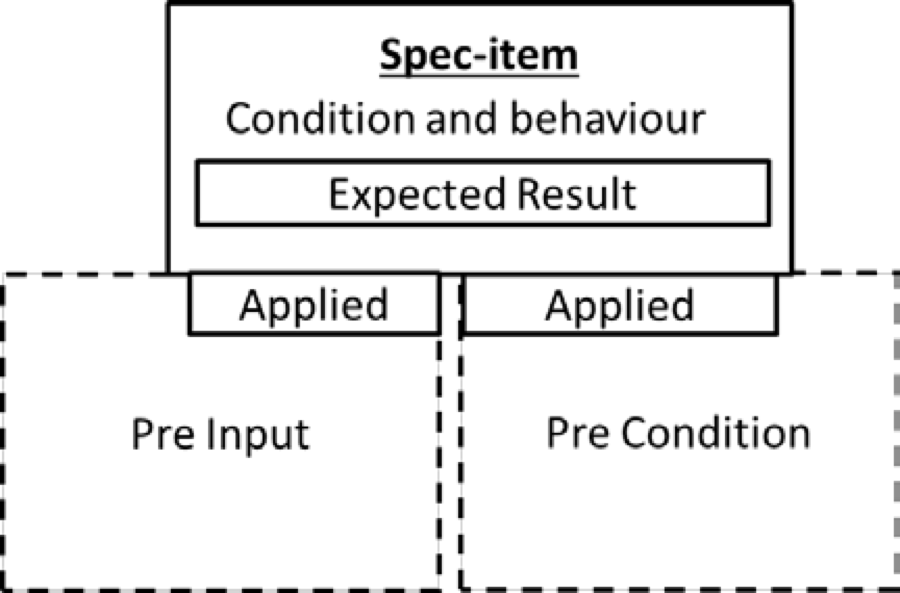
\includegraphics[width=10cm]{./image/D-4-Fig1.png}
  \caption{テスト条件の構成要素}
  \label{fig:D-4-Fig1}
  \end{center}
   \end{figure}

このテスト条件を合理的にある基準で網羅する方法を考える行為がテスト設計であり,そのための技法をテスト設計技法と呼ぶ.
テスト設計のアウトプットはテストケースである.

\begin{figure}[h]
  \begin{center}
  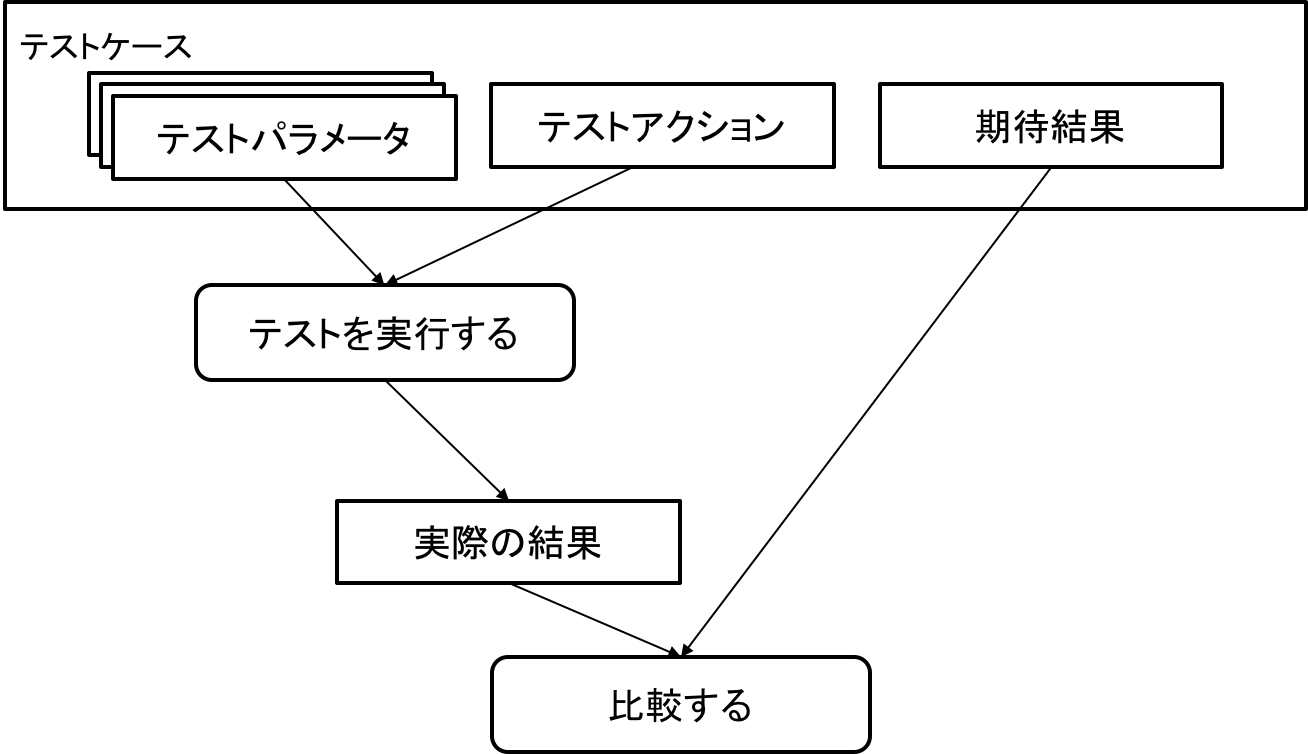
\includegraphics[width=10cm]{./image/D-2-FigTCS.png}
  \caption{テストケースを実行するプロセス}
  \label{fig:D-4-FigTCS}
  \end{center}
\end{figure}

IEEE610では,テストケースを,特定の目的のために開発されたテスト入力,実行条件,期待結果の3つで構成されると定義している.
また,機能テストは,選択した入力と実行条件のレスポンスとして生成されたアウトプットを確認する,と定義している\cite{IEEE610}.
すなわち,機能テストとは,ブラックボックステストと同義である.
テスト入力,実行条件には,事前に設定されているものと,実行時点で設定するものがある.
おのおのは,表~\ref{tab:D-4-FigTPS}に示すよう分類できる.
その上で,本研究では,事前入力と事前条件をまとめたものをテストパラメータ,イベントと操作をまとめたものをテストアクションと呼ぶこととする\cite{yumoto2013-a}.
テスト条件を網羅するテストケースを開発する際,テストアクションはテスト対象を動作させてアウトプットを導く直接的な要因である.
そのため,テスト実行にてアウトプットを導くテストアクションは1つに特定できる.
テストパラメータは,1つのテストアクションに対して多くのバリエーションを取り得る.

% Table generated by Excel2LaTeX from sheet '論文挿絵'
\begin{table}[htbp]
  \centering
  \caption{テストの構成要素の再分類}
    \begin{tabular}{|l|l|l|}
    \hline
          & 事前に設定 (パラメータ)  & 実行時点で設定 (アクション)  \bigstrut\\
    \hline
    テスト入力  & 事前入力  & イベント  \bigstrut\\
    \hline
    実行条件  & 事前状態  & 操作  \bigstrut\\
    \hline
    \end{tabular}%
  \label{tab:D-4-FigTPS}%
\end{table}%

ブラックボックステストのテストケースとテスト実行をするプロセスを図示すると,図~\ref{fig:D-4-FigTCS}のように表すことができる.
テスト入力,実行条件となるテストパラメータ,テストアクションを入力としてテストを実行し,出力した実際の結果が期待結果と一致するかを比較する.期待と一致すればテストは成功であり,期待と一致しなければ,インシデントとして報告することになる.




\newpage
\section{テスト対象詳細化の問題} \label{sec:2-2}
\subsection{分類に対する一貫性の欠如}
テスト分析の活動の出力となるテスト条件は,「機能,トランザクション,品質特性,構造的要素\cite{ISTQB}」といったアプリケーションソフトウェアの側面の総称である.
これらの側面について記述した成果物は,仕様である.
ブラックボックステストのテスト分析では,これらの側面が記述されている仕様に対して,テスト対象をテストケースが作れるサイズまで詳細化していく.
詳細化する際は,テスト対象の詳細化をするときの起点や中間分類が人によって異なってバラバラになってしまわないように分類の関係を整理する必要がある.
しかし,実務において,テスト分析におけるテスト条件群の整理方法は,経験則や個人の考え方に基づいている.

一般的には,テストベースを大項目,中項目,小項目と詳細化していくことが多い.
この方法は,詳細化する際の各分類項目に当てはめるアプリケーションソフトウェアの側面に明確なルールが定義されていないため,個人毎の何かしらの考え方で詳細化するための分類を決めていくことになる.
そのため,複数人で作業を行うと分類にばらつきが発生し,同じ項目が複数の階層に現れてしまったり,同じ意味の項目が別の名称で選択されるといった混乱を引き起こす.
混乱が起きている例を表~\ref{tab:analysissample}に示す.
% Table generated by Excel2LaTeX from sheet '論文挿絵'
\begin{table}[htbp]
  \centering
  \caption{一般的なテスト分析の詳細化の例}
    \begin{tabular}{|l|l|l|l|p{5em}|p{6em}|}
    \hline
    大項目   & 中項目   & 小項目   & 細目    & 補足項目  & テスト条件 \bigstrut\\
    \hline
    印刷    & 設定    & 印刷部数  & --    & --     & 100部印刷した場合 \bigstrut\\
    \hline
    設定    & プリント設定 & 一般    & 異常系   & \shortstack{エラー\\メッセージ} & 「印刷部数が99部を超えました」と表示されること \bigstrut\\
    \hline
    \end{tabular}%
  \label{tab:analysissample}%
\end{table}%

表~\ref{tab:analysissample}の例には,以下のような問題がある.
\begin{enumerate}
\item 設定というカテゴリが大項目に出ている場合と中項目に出ている場合が混在している.
\item 階層数も一定でないため,各階層がどのような意味を持つものかがばらついている.
\item 上段は,期待結果が書かれていない.
\item 上段と下段は同じテスト条件について書かれている.
\end{enumerate}
テスト開発の最初の活動であるテスト分析にて,詳細化で現れる項目の内容にこのような問題があると,その後の活動で作られるテストケースの抜け漏れ,重複に影響を及ぼす可能性が高くなると考えられる.
このような課題については,Eldhが,「指示内容理解(Understanding Instruction)」の不足によるテストケースの品質低下について調査をしており,複数の解釈による間違いが起きることを報告している\cite{eldh2011analysis}.

ISTQBでは,テスト分析の活動を「…テスト分析の期間中,何をテストするか決定するため,すなわち,テスト条件を決めるために,テストのベースとなるドキュメントを分析する」と説明している.
しかし,この説明は,テスト分析を実行するための要求事項や必要性は述べているだけであり,テストベースを分析していくための方法を具体的に定義していない.
Ostrand\cite{Ostrand:1988:CMS:62959.62964}, Grindal\cite{Grindal:2007:IPM:1332044.1332085}などのテストケースの開発に関する先行研究は,テスト分析にてテスト条件が特定された後のテスト設計で行われるテストパラメータの設計に焦点を当てている.
それらの研究では,テスト条件は,すでに全て準備されたと言う前提になっている.
テスト分析手法に関する研究は,Nishi\cite{nishi2012based}, Akiyama\cite{Akiyama2014}がある.
しかし,複数の人数でテストケースを作る際に起きる課題については言及していない.

\newpage
\section{機能間の統合に対するテストケース作成の問題} \label{sec:2-3}
\subsection{既存の網羅基準によるテストケース数の増大}
テストケース数の増加は,単一機能のテストより機能間の統合において問題となる.
この場合のテストケース数は,単一の機能や制御構造の和で求めるのではなく,積となるためである.
それに加え,複数機能を統合したもののテストでは,状態遷移に伴う時系列の組合せのテストも求められることから,テストケース数の爆発問題が生じる.
必要なテストケースの抽出方法とその網羅性に関する手法は,多くは機能や制御構造を基にした方法である.
そのため,機能間の統合と状態遷移に伴う時系列の組み合わせには対応していない.

状態遷移間の組合せについては,Nスイッチカバレージに従ってテストケースを抽出する方法がある \cite{chow1978testing}\cite{whittaker1994markov}\cite{lee1996principles}\cite{fujiwara1991test}\cite{andrews2005testing}.
Nスイッチカバレージでは,状態の遷移をパスとし,N+1 個の遷移パスを網羅する基準に従て組合せテストケースを作成する.
N=0 では遷移パスの組合せをテストできないため N=1,すなわち S1網羅基準(1スイッチカバレージ)が必要とされている.
しかし,S1網羅基準を満たすテストケース数は,2つの状態遷移間における遷移数の積となり,膨大なテスト工数が必要となる.

S1網羅基準の課題に対するアプローチとしては,自動化により工数を削減する研究とテストケース数を削減する先行研究がある.
自動化による工数削減の研究は,N-スイッチカバレージを満たすテストケースを形式仕様から自動生成する方法が知られている.
この方法は,テスト対象となるITシステムの動作を正確に記述したモデルを定義し,そのモデルから特定の長さの連続した遷移を抽出する方法である\cite{takagi2010concurrent}.
対象システムが運動方程式などに従う一般的なモデルベーステストと異なり,状態遷移にて生ずるシステムの動的な振舞いを形式仕様化する必要があり,それが困難であることから一般的なITシステムで適用された例は見当たらない.
生成されるテストケース数はN-スイッチカバレージと同じであり削減されないので,テストケースが自動抽出されても,実行のための操作は人手に頼る部分が残り,作業工数を合理化できない課題がある.

テストケース数を削減する研究としては,状態遷移の組合せに対して直交表を応用し2因子間の組合せを中心に,一部3因子の組合せも抽出する研究がある\cite{akiyama2007}\cite{akiyama2012}.
この方法は,決定表を用いて機械的に組合せを抽出でき,2因子間の組合せ即ちS0網羅基準は完全に網羅できるが,S1 網羅基準の網羅は不完全であり,かつその選択基準が用いた直交表に左右されるため重要なテストケースが漏れる課題がある.

現実的な方法としては,設計で用いられるUMLのシーケンス図を基にテストケースを抽出する方法が知られている\cite{hartmann2000uml}.
この方法によるテストケース数はシーケンス図で定義されたシーケンスで決まる.
シーケンス図が状態遷移のS1網羅基準を満たすか否かは,シーケンス図が表すテスト対象のサブセットの範囲による.
多くの場合,設計者が意図したシーケンスは,起こり得る状態遷移の組合せの一部しか表してないため,漏れが生じる課題がある.

\newpage
\section{テストカテゴリベースドテスト}
本研究では,テストカテゴリベースドテスト\cite{yumoto2013test}というテスト分析手法を利用した予備実験を行い,テスト分析の課題の調査,およびテスト分析の知識を与えることによるテストケースを網羅的に抽出できるスキル向上傾向の調査を行なった.
この結果は3章に記載をする.
この分析手法を使って調査を行う理由は,以下のとおりである.
\begin{enumerate}
\item 前述したテスト分析の問題のうち,分類に対する一貫性の欠如を解決するために自身で提案し,現場にて適用している手法である.
\item 検証実験のための題材となる仕様書,模範解答が揃っており,それらの題材を使って実験を行った研究結果がある.
\item 本研究で合理的にテストケースの抽出を行う手法を提案する基の考え方として,テストカテゴリベースドテストを基にしていることである.
\end{enumerate}

本節では,テストカテゴリベースドテストの概要を説明する.
このテスト分析手法のアプローチでは,テスト対象のサブセットに属するタスクの仕様項目を特定していく方法を提示する.
また,テストケースの構造をベースにテスト条件を分解することで,テスト条件と言う用語の持つ曖昧さを排除する.
タスクとは,前述した通り,アプリケーションソフトウェアにて何らかの入力を出力に変換する処理のことである.
また,階層の要素としてテストカテゴリという,テスト対象の知識と欠陥と故障の知識を使って定義した分類を構造に追加している.

\subsection{テスト条件群の構造}
前述した通り,テスト条件とは,機能,トランザクション,品質特性,構造的要素といったアプリケーションソフトウェアの側面の総称である.
通常,これらはアプリケーションソフトウェアの仕様として記載されるものである.
ブラックボックステストにおけるテスト条件群をテストケースの構成要素で整理すると,図~\ref{fig:D-4-Fig4}に示した構造で整理できる.

\begin{figure}[htbp]
  \begin{center}
  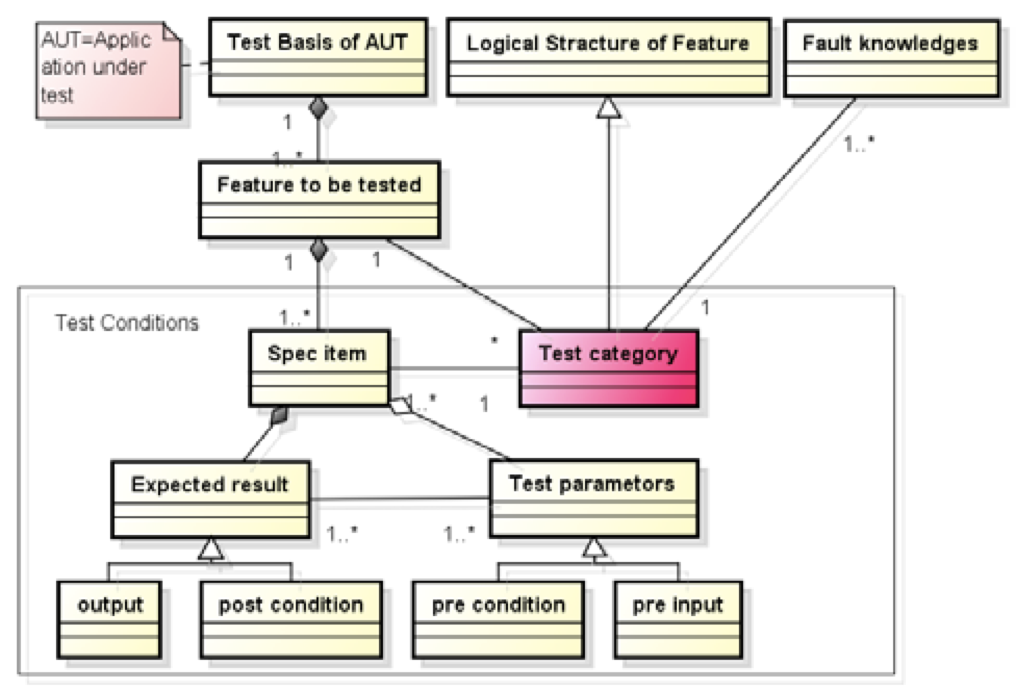
\includegraphics[width=10cm]{./image/D-4-Fig4.png}
  \caption{テストケースの構成要素で整理したテスト条件の構造}
  \label{fig:D-4-Fig4}
  \end{center}
   \end{figure}

テストベースは,テストケースを抽出する基になる文書のことであり,開発時に作成する要件や設計内容が書かれた文書が該当する.
テストベースにはフィーチャを実現するタスクを明確に定義する仕様項目が1つ以上記述されている.
フィーチャとは,利用者が観察可能なソフトウェアシステムの論理的なサブセットであり,利用者とテスト対象のインターフェースとなる\cite{kang1990feature}.
ブラックボックステストは,外部観察によるテスト設計の方法であるため,テスト条件をフィーチャから選択することが必要になる.
テスト対象となるフィーチャはISO/IEC/IEEE29119の定義に従い,フィーチャセットと呼ぶ\cite{ISO29119}.

仕様項目とは,フィーチャセットに属するタスクの要件を綿密に定義し文書化したものである.
タスクの要件とは,フィーチャセットの振る舞いのひとつであり,例えば「ボリュームは1から10の間で設定できる.1は消音であり,10は100dbsになる」が該当する.
この記述が仕様項目である.
テスト分析では,テストすべき仕様項目を特定していく.
その仕様項目の内容をテストケースの構成と同じように期待結果とテストパラメータに分類し,整理する.
テストパラメータとは,テストケースの構成要素のひとつで,事前入力と事前条件を汎化したものである.
期待結果は,出力と事後条件を汎化したものである.
このような分類,整理によって,明確なルールにそったテスト分析が可能になる.

\subsection{論理的機能構造}
ブラックボックステストの場合,テスト対象の内部構造を完全に知ることはできなく,テスト実行は入力と出力だけが頼りになる.
大村は「…人工のシステムとは,インプットを変換し付加価値を与えアウトプットする変換装置であるため,論理的には,必ず図~\ref{fig:D-2-FigLSOF}のような構造を持つ\cite{LSOF}」と主張している.
\begin{figure}[htbp]
  \begin{center}
	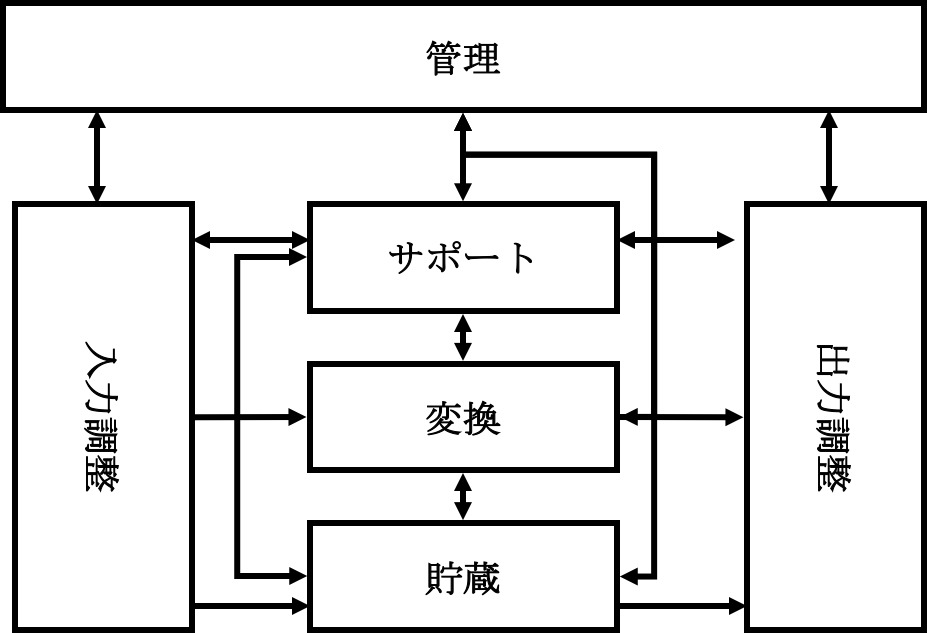
\includegraphics[width=10cm]{./image/D-2-FigLSOF.png}
	\caption{人工システムの論理構造}
	\label{fig:D-2-FigLSOF}
  \end{center}
\end{figure}

\begin{description}
  \item[入力調整]入力される資源は,直接変換機能に送り込まれることなく,変換しやすいように入力機能によって整えられたのちに送り込まれる.
  \item[出力調整]不十分であったり不必要なものを含む変換されて出てくる資源をシステムから出力する前に,有用資源に調整したり不必要なものを始末する.
  \item[変換]システムの中核となる基本機能.システムが目的を達成するのに直接関わり,システムを特徴付ける.
  \item[貯蔵]入力資源を変換機能に安定的に供給したり,出力資源を外部の要求に合わせて送り出すために,さらには他の基本機能がスムーズに働くためにシステム内に資源を蓄える.
  \item[サポート]変換をはじめとする他の機能が円滑に働くために、それぞれの機能を裏から支える.
  \item[管理]変換装置全体が様々な制約の中で秩序関係を維持しながら目的を達成できるようにする.
\end{description}


テストカテゴリベースドテストは,同様のコンセプトを利用している.
つまり,テスト対象となるフィーチャセットは同様の論理構造を持つ人工システムだと捉える.
この論理構造を,フィーチャをMECE(互いに相容れなくて完全に徹底的)\cite{ethan1999mckinsey}な方法でテストをするために利用する.
テストカテゴリベースドテストでは,人工システムが持つ論理構造を基にして,図~\ref{fig:D-3-Fig3}のように定義し,論理的機能構造と命名する.

図~\ref{fig:D-3-Fig3}に示す各箱は,テスト対象の内部構造を推定し,テストが必要なタスクを特定する有用なモデルとして利用できる.
そして,タスクに関する記述がされている仕様項目がテスト条件となる.
\begin{figure}[htbp]
  \begin{center}
	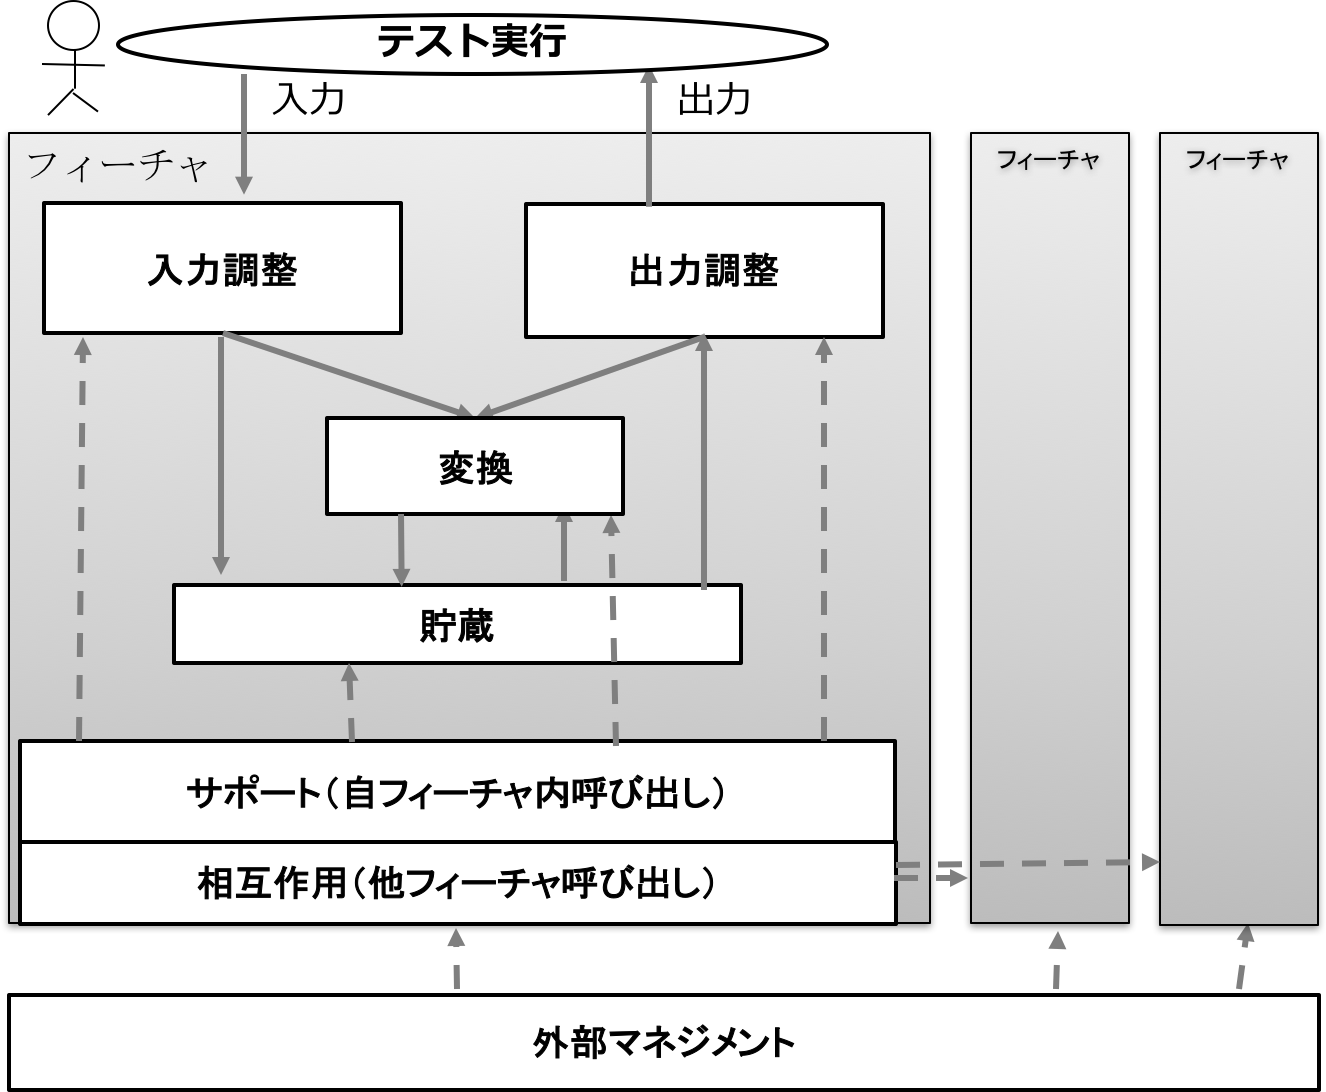
\includegraphics[width=10cm]{./image/D-3-Fig3.png}
	\caption{論理的機能構造}
	\label{fig:D-3-Fig3}
  \end{center}
\end{figure}

テスト分析をしていく際に論理的機能構造を使って内部構造を推定してタスクを特定していく方法を導入すると,テストに必要なテスト条件の特定が容易になるという仮説を立てている.
現状,次に示す課題はテスト条件の特定を困難にしている.

\begin{enumerate}
\item 明白に必要だと思われる仕様の一部分が記述されていない.
\item 機能間の組み合わせでどのように振舞うかといった仕様は,テストベース中の該当する単一の節以外に記載される.
\end{enumerate}

\subsection{テストカテゴリ}
論理的機能構造は抽象的な概念であるため,テスト分析をするそれぞれの技術者の間にて解釈の違いが生じる可能性がある.
テスト条件を決定する際に,その解釈に一貫性を持たせるため、論理的機能構造の箱に対してテスト対象で使われる用語を使った名前付けをする.
そのようなテスト対象に特化して付けた論理的機能構造の各箱の名前をテストカテゴリと呼ぶ.
テストカテゴリはテスト条件を特定するための有用なガイドである.
特定したテスト条件にはフィーチャセットの仕様項目,期待結果,テストパラメータが含まれている.
決定したテストカテゴリは,テストケースの作成に携わる各人員がテストカテゴリの意味を同じように理解していることを確認する必要がある.

\begin{table}[htbp]
  \centering
  \caption{テストカテゴリ一覧の例}
    \begin{tabular}{|p{6em}|p{8.07em}|p{14.645em}|}
    \hline
    \textbf{論理的構造} & \textbf{テストカテゴリ} & \textbf{意味づけ(想定する欠陥)} \bigstrut\\
    \hline
    \multirow{2}[4]{*}{\textbf{入力調整}} & \textbf{画面入力} & \textbf{入力チェック,入力画面の制御} \bigstrut\\
\cline{2-3}    \multicolumn{1}{|l|}{} & \textbf{ボタン操作} & \textbf{画面遷移のルール,処理起動} \bigstrut\\
    \hline
    \textbf{出力調整} & \textbf{表示} & \textbf{処理結果の表示,出力数の制御} \bigstrut\\
    \hline
    \multicolumn{1}{|r|}{} & \textbf{帳票出力} & \textbf{印刷内容,印刷フォーマット} \bigstrut\\
    \hline
    \textbf{変換} & \textbf{計算} & \textbf{料金計算} \bigstrut\\
    \hline
    \multirow{2}[4]{*}{\textbf{貯蔵}} & \textbf{検索} & \textbf{検索条件の組み合わせ,検索結果} \bigstrut\\
\cline{2-3}    \multicolumn{1}{|l|}{} & \textbf{登録/更新/削除} & \textbf{DB処理} \bigstrut\\
    \hline
    \textbf{相互作用} & \textbf{反映} & \textbf{DB処理結果の他機能への反映} \bigstrut\\
    \hline
    \textbf{サポート} & \textbf{エラー処理} & \textbf{エラー復旧処理} \bigstrut\\
    \hline
    \end{tabular}%
  \label{tbl:D-4-tbl1}%
\end{table}

各テストカテゴリに分類したテストにて発見する可能性のある欠陥および故障を,例を挙げてディスカッションし,
その結果を表~\ref{tbl:D-4-tbl1}で示した表にまとめる.
ディスカッションにより,テスト開発プロセス活動にかかわるメンバーは,テストカテゴリの意味に対して合意形成をすることができる.
合意形成のねらいは次のとおりである.

\begin{enumerate}
\item テスト開発にかかわるテスト担当がフィーチャセットに対して同様の理解に達することができる.
\item テスト担当間のテスト条件の解釈のぶれを最小限にとどめることができる.
\end{enumerate}


\subsection{実施手順}
構造化したテスト条件群を順番に導くために,テスト分析の活動を図~\ref{fig:D-4-Fig3}のような作業ステップに分割し,各ステップでのインプットとアウトプットを定義する.


\begin{figure}[htbp]
  \begin{center}
  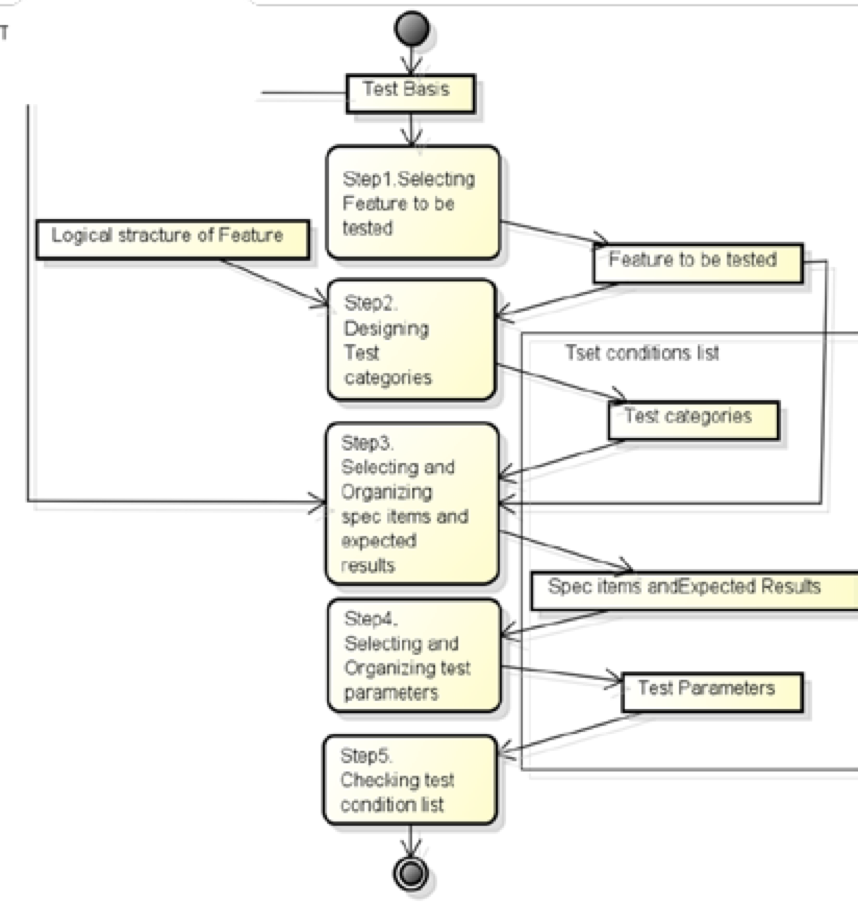
\includegraphics[width=12cm]{./image/D-4-Fig3.png}
  \caption{テスト分析の実行ステップ}
  \label{fig:D-4-Fig3}
  \end{center}
   \end{figure}


以降に各作業ステップについて説明をする.

\begin{description}
\item[Step1] フィーチャセットを選択

テストベースからテスト対象のサブセットとなるフィーチャセットを特定する.
フライト予約をするアプリケーションソフトウェアで例えた場合,新規フライト予約(搭乗したい飛行機の条件を照合し,予約を成立させる一連の機能群)がフィーチャセットとなる.

\item[Step2] テストカテゴリの設計

テストカテゴリを設計する方法は,階層ホログラフィックモデリング法(HHM法)におけるサブトピックの設定方法と類似している\cite{HHM2002}.
HHM法でいうところのメイントピックにフィーチャセットを置く.
メイントピックを構成するサブトピックとして論理的構造毎にフィーチャセットの動作条件や振る舞いを列挙する.
列挙する際はどのような欠陥および故障が起きることが考えられるかを検討材料にして列挙する.
選択したフィーチャセット全部に対してサブトピックを列挙した後に,サブトピック全体を眺めて,象徴する名称を付与し,それをテストカテゴリにする.
テストカテゴリは,メンバ間で内容を説明し,意味づけ(どのような欠陥および故障が起きるか)を共有することで,解釈のぶれを防ぐ.


\item[Step3] テストカテゴリを使い仕様項目と期待結果を特定,整理する.

テストカテゴリでフィーチャの内部構造を推定し,実現するタスクを特定する.
テストベースからそのタスクの仕様項目と期待結果の記述を抽出する.


\item[Step4] テストパラメータを選択し,整理する.

特定した仕様項目と期待結果からテストパラメータを選択する.テストパラメータは特定した仕様項目と期待結果にに沿ってテストベースを分析して選択する.

\end{description}



% Table generated by Excel2LaTeX from sheet 'Sheet2'
\begin{table}[htbp]
  \centering
  \caption{テスト条件一覧の例}
    \begin{tabular}{|c|p{6em}|p{6em}|p{6em}|p{7.145em}|}
    \hline
    \multicolumn{1}{|p{8.855em}|}{\textbf{フィーチャセット}} & \textbf{テストカテゴリ} & \textbf{仕様項目} & \textbf{期待結果} & \textbf{テストパラメータ} \bigstrut \\
    \hline
    \multicolumn{1}{|c|}{\multirow{4}[8]{*}{TF-a}} & TC-a  & SI-a  & ER-a  & TP1,TP2 \bigstrut\\
\cline{2-5}          & \multicolumn{1}{l|}{} & SI-b  & ER-b-1 & TP1,TP3,TP4 \bigstrut\\
\cline{2-5}          & \multicolumn{1}{l|}{} & \multicolumn{1}{l|}{} & ER-b-2 & TP1,TP4 \bigstrut\\
\cline{2-5}          & TC-b  & SI-c  & ER-c  & TP5,TP6,TP7 \bigstrut\\
    \hline
    \multicolumn{1}{|c|}{\multirow{2}[4]{*}{TF-b}} & TC-a  & SI-d  & ER-d  & TP9,TP10 \bigstrut\\
\cline{2-5}          & TC-b  & N/A   & N/A   & N/A \bigstrut\\
    \hline
    \end{tabular}%
  \label{tbl:D-3-tbl3}%
\end{table}%

テストベースからテスト条件を特定する際は,その結果を表~\ref{tbl:D-3-tbl3}に示すテスト条件リストにまとめる.

テスト条件一覧の最初の列には,フィーチャセットを列挙する.
各フィーチャセットの隣には,テストカテゴリのセットを列挙する.
そして,各テストカテゴリに対応する仕様項目と期待結果を列挙する.
フィーチャセットによってはテストカテゴリに対応する仕様項目が無い場合もある.
その場合はテストカテゴリの中に列挙されるものが何も無いため,N/Aと記載する.


仕様項目によっては,期待結果が複数になることがある.
その際は,1つの仕様項目に対して複数の期待結果を記載する.
テストパラメータには,各仕様項目と期待結果のセットから見て適切なテストパラメータの組み合わせを選択する.
テストパラメータは,テスト分析の後の活動となるテスト設計にて同値分割を行い適切な同値クラスにする.
複数の同値分割の組み合わせは,ディシジョンテーブル技法やペアワイズテスト技法を使って
適切な組み合わせを設計する.

多くのテストケースの開発に従事するテスト担当者が上記のステップに従うと,同じルールに沿って分析を行うことができる.
結果として,特定したテスト条件の一覧は,包括的で,重複が含まれない.
このようなテスト条件一覧を作成することは,高いテストカバレッジを確かにし,高品質なテストを提供することにつながる.
これは本手法の主たる効果となる.
更に,この手順にしたがってテスト分析を行うことには3つの効果がある.

\begin{enumerate}
\item この手順は,図~\ref{fig:D-4-Fig4}で示した「テストケースの構成要素で整理したテスト条件の構造」
をベースにしている.この手順を通して,テストベースを仕様項目,期待結果,テストパラメータをそれぞれ順番に特定,選択していく.
テストケースの開発に携わる人員は,テスト分析の活動を通じて同じ順番でテスト条件を特定し同じカテゴリに分類できるため,全員の成果物をまとめて確認する際の可読性が向上する.
\item テストカテゴリに対する合意形成によって,テストケースの開発に携わる人員は仕様項目の特定と選択を同じ認識を持って行える.人員間での情報共有も容易になる.
\item 本手法は体系化,標準化して進めていくのが容易になるため,組織に関わるテストケースの開発に携わる人員がテスト分析を繰り返すことができるようになる.
\end{enumerate}

\subsection{テスト条件特定結果の比較}

テストケースの開発に関するワークショップを開催し,同一組織内にてソフトウェアテストに従事している人員で2チームに分かれて,テストカテゴリベースドテストの説明で記した「テスト分析の作業Step3:テストカテゴリを使った仕様項目と期待結果の選択」の演習を行った.

1つのチームは,テストカテゴリを使わずに仕様項目,期待結果,テストパラメータを列挙してもらい,もう1つのチームは,テストカテゴリを使って仕様項目,期待結果,テストパラメータを列挙してもらった.題材として音楽再生機器を選定した.出席者は全て類似の機器のシステムテストに関わった経験があり,製品知識はある.
フィーチャセットは,音楽再生機器のボリュームコントロール機能である.

2つの演習結果と演習の模範解答を比較し,解答例と同じだけの仕様項目を特定できれば網羅的に分析ができているとする.
また,テストカテゴリベースドテストを適用した場合とそうでない場合の違いを分析した.
グループの回答を比較データに使った理由は,この手法の効果が複数の人員でテスト分析をしたときのばらつきからくる欠損や重複を防ぐことを狙っているためである.

% Table generated by Excel2LaTeX from sheet '集計 (J)'
\begin{table}[htbp]
  \centering
  \caption{仕様項目の選択割合の比較}
    \begin{tabular}{|l|r|r|r|r|r|r|r|r|r|r|r|r|}
    \hline
          & \multicolumn{1}{p{2em}|}{入力調整} & \multicolumn{2}{c|}{変換} & \multicolumn{2}{p{3em}|}{サポート} & \multicolumn{2}{p{2em}|}{出力調整} & \multicolumn{2}{c|}{貯蔵} & \multicolumn{1}{p{2em}|}{相互作用} & \multicolumn{1}{l|}{\textbf{合計}} & \multicolumn{1}{l|}{\textbf{比率}} \bigstrut\\
    \hline
    解答例   & 0     & 2     & 1     & 0     & 2     & 1     & 0     & 1     & 0     & 2     & 9     & 100\% \bigstrut\\
    \cline{1-13}
    \multicolumn{1}{|p{7em}|}{テストカテゴリ未適用}  & 0     & 2     & 0     & 0     & 0     & 1     & 0     & 1     & 0     & 1     & 5     & 56\% \bigstrut\\
    \cline{1-13}
    \multicolumn{1}{|p{7em}|}{テストカテゴリ適用}  & 0     & 2     & 0     & 0     & 2     & 1     & 0     & 1     & 0     & 1     & 7     & 78\% \bigstrut\\
    \hline
    \end{tabular}%
  \label{tab:addlabel6}%
\end{table}%

演習結果にて,仕様項目の選択数を比較すると表~\ref{tab:addlabel6}のようになった.
1番上の行は解答例であり,講師が予め準備したものである.
2番目と3番目の行はワークショップの中で各チームが演習中に作成したものである.
テストカテゴリを利用したチームは講師と同じテストカテゴリを利用し,テストカテゴリを利用していないチームは,演習後にこちらでテストカテゴリにマッピングして比較可能にした.
両方のチームとも解答例と同じ数の仕様項目の特定はできなかった.
チーム間の比較をした場合,テストカテゴリありのチームのほうが仕様項目の選択割合が2つ多く,より高い結果となった.

また,各仕様項目として列挙した期待結果とテストパラメータ数の集計は表~\ref{tab:D-2-resilt2}のような結果となった.

% Table generated by Excel2LaTeX from sheet '集計 (J)'
\begin{table}[htbp]
  \centering
  \caption{期待結果とテストパラメータ数の選択結果}
    \begin{tabular}{|l|r|r|r|r|r|r|}
    \hline
    \multirow{2}[4]{*}{テストカテゴリ} & \multicolumn{2}{c|}{仕様項目} & \multicolumn{2}{c|}{期待結果数} & \multicolumn{2}{c|}{パラメータ数} \bigstrut\\
\cline{2-7}          & \multicolumn{1}{l|}{適用なし} & \multicolumn{1}{l|}{適用あり} & \multicolumn{1}{l|}{適用なし} & \multicolumn{1}{l|}{適用あり} & \multicolumn{1}{l|}{適用なし} & \multicolumn{1}{l|}{適用あり} \bigstrut\\
    \hline
    入力A   &       &       & \multicolumn{1}{l|}{N/A} & \multicolumn{1}{l|}{N/A} & \multicolumn{1}{l|}{N/A} & \multicolumn{1}{l|}{N/A} \bigstrut\\
    \hline
    \multirow{2}[4]{*}{変換A} & \multicolumn{1}{c|}{○} & \multicolumn{1}{c|}{○} & 1     & 1     & 5(3)  & \multicolumn{1}{l|}{N/A} \bigstrut\\
\cline{2-7}          & \multicolumn{1}{c|}{○} & \multicolumn{1}{c|}{○} & \multicolumn{1}{l|}{N/A} & 1     & 1     & \multicolumn{1}{l|}{N/A} \bigstrut\\
    \hline
    変換B   &       &       & \multicolumn{1}{l|}{N/A} & \multicolumn{1}{l|}{N/A} & \multicolumn{1}{l|}{N/A} & \multicolumn{1}{l|}{N/A} \bigstrut\\
    \hline
    サポートA &       &       & \multicolumn{1}{l|}{N/A} & \multicolumn{1}{l|}{N/A} & \multicolumn{1}{l|}{N/A} & \multicolumn{1}{l|}{N/A} \bigstrut\\
    \hline
    \multirow{2}[4]{*}{サポートB} &       & \multicolumn{1}{c|}{○} & \multicolumn{1}{l|}{N/A} & 1     & \multicolumn{1}{l|}{N/A} & 2 \bigstrut\\
\cline{2-7}          &       & \multicolumn{1}{c|}{○} & \multicolumn{1}{l|}{N/A} & 1     & \multicolumn{1}{l|}{N/A} & 2 \bigstrut\\
    \hline
    出力A   & \multicolumn{1}{c|}{○} & \multicolumn{1}{c|}{○} & 1     & 1     & \multicolumn{1}{l|}{N/A} & 2 \bigstrut\\
    \hline
    出力B   &       &       & \multicolumn{1}{l|}{N/A} & \multicolumn{1}{l|}{N/A} & \multicolumn{1}{l|}{N/A} & \multicolumn{1}{l|}{N/A} \bigstrut\\
    \hline
    貯蔵A   & \multicolumn{1}{c|}{○} & \multicolumn{1}{c|}{○} & 1     & 1     & 3(1)  & 2 \bigstrut\\
    \hline
    貯蔵B   &       &       & \multicolumn{1}{l|}{N/A} & \multicolumn{1}{l|}{N/A} & \multicolumn{1}{l|}{N/A} & \multicolumn{1}{l|}{N/A} \bigstrut\\
    \hline
    \multirow{2}[4]{*}{相互作用A} & \multicolumn{1}{c|}{○} & \multicolumn{1}{c|}{○} & \multicolumn{1}{l|}{N/A} & 1     & 1     & 1 \bigstrut\\
\cline{2-7}          &       &       & \multicolumn{1}{l|}{N/A} & \multicolumn{1}{l|}{N/A} & \multicolumn{1}{l|}{N/A} & \multicolumn{1}{l|}{N/A} \bigstrut\\
    \hline
    合計    & 5     & 7     & 3     & 7     & 10(4) & 9(0) \bigstrut\\
    \hline
    \end{tabular}%
  \label{tab:D-2-resilt2}%
\end{table}%


テストカテゴリを利用しなかったチームは,期待結果が明記されていなく,テストパラメータをあらわすテスト条件のみ記載している仕様項目がテストカテゴリを利用したチームと比較して4つ多かった.
列挙されていたパラメータ数は,テストカテゴリを利用しないチームのほうが11多く,4倍以上であった.
また,テストパラメータの内容を被験者に確認して,同じ仕様項目のパラメータになるものが別の仕様項目として記述されていたものを講師が集計時に分類し直した.パラメータ数の欄に()にて記した.
テストカテゴリを利用しないチームは,パラメータ数の欄に()で記した数が4つあった.
これらはテスト設計時に重複したテストケースを設計してしまう可能性がある.

\section{まとめ}
本章では,研究の対象となるアプリケーションソフトウェア,テストケースの種類,テストレベル,テストプロセスを明記し,ソフトウェアテストの中で,システムテストレベルでのブラックボックステストを研究の対象にすること,ブラックボックステストのテストケースを開発する活動の中では,テスト分析を対象にすることを述べた.
そして,そこで起きている問題として,テスト対象を詳細化するときに分類に対する一貫性が欠如していることを述べた.また,機能間の統合に対する問題として,既存の網羅基準を適用するとテストケース数が膨大になることを述べた.

これらの問題に対して,テストカテゴリベースドテストというテスト分析手法を基に研究をすすめるため,前提知識としてこの手法の概要と,既出の実験結果を説明した.
